\section{Results}\label{sec:results}

Unless stated otherwise, results use Protocol~I, 300 evaluated accounts, 400 donor accounts and master seed 20260920. Figures and tables are generated from the files in the repository's \texttt{results/} directory.

\subsection{Data-Efficiency Curves on Real Histories}\label{sec:curves}

\begin{figure}[!t]
\centering
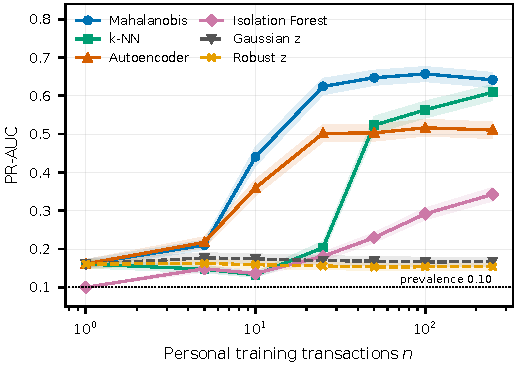
\includegraphics[width=\columnwidth]{figures/fig_berka_curves.pdf}
\caption{Data efficiency on real bank histories (Berka, Protocol~I, 300 accounts). PR-AUC of six personal detectors against the number of personal training transactions $n$; shaded bands are 95\% bootstrap intervals over accounts. Mahalanobis distance and the autoencoder rise steeply and saturate early, $k$-NN rises sharply between $n=25$ and $50$, and the two univariate $z$-scores stay flat at every size.}
\label{fig:berka}
\end{figure}

\begin{table}[!t]
\caption{Mean PR-AUC of personal detectors on Berka (Protocol~I, 300 accounts; prevalence baseline 0.100). Best per row in bold; ties at $n=1$ not marked.}
\label{tab:berka}
\centering\footnotesize\setlength{\tabcolsep}{3.2pt}
\begin{tabular}{r cccccc}
\toprule
$n$ & Mahal. & $k$-NN & Autoenc. & IForest & Gauss.\ z & Robust z \\
\midrule
1   & 0.161 & 0.161 & 0.161 & 0.100 & 0.161 & 0.161 \\
5   & 0.210 & 0.147 & \textbf{0.218} & 0.149 & 0.177 & 0.162 \\
10  & \textbf{0.441} & 0.132 & 0.360 & 0.136 & 0.174 & 0.159 \\
25  & \textbf{0.625} & 0.204 & 0.502 & 0.181 & 0.170 & 0.156 \\
50  & \textbf{0.647} & 0.523 & 0.503 & 0.230 & 0.168 & 0.153 \\
100 & \textbf{0.657} & 0.563 & 0.517 & 0.292 & 0.166 & 0.153 \\
250 & \textbf{0.642} & 0.609 & 0.511 & 0.343 & 0.167 & 0.153 \\
\bottomrule
\end{tabular}
\end{table}

\begin{table}[!t]
\caption{Saturation fits and sufficiency thresholds on Berka. Fits are $y(n)=y_{\max}-(y_{\max}-y_0)e^{-n/\tau}$. Rel-90 and Rel-95 are the relative thresholds of \cref{sec:protocol}; a dash means the criterion is never met on the evaluated grid.}
\label{tab:thresholds}
\centering\footnotesize\setlength{\tabcolsep}{3.5pt}
\begin{tabular}{l ccc ccc}
\toprule
Detector & $y_{\max}$ & $\tau$ & $R^2$ & Rel-90 & Rel-95 & Stability \\
\midrule
Mahalanobis      & 0.658 & 11.5 & 0.970 & 25  & 25  & --- \\
Autoencoder      & 0.518 & 11.1 & 0.980 & 25  & 25  & --- \\
$k$-NN           & 0.633 & 50.9 & 0.912 & 100 & 250 & --- \\
Isolation Forest & 0.350 & 71.2 & 0.985 & 250 & 250 & --- \\
Robust z         & 0.153 & 21.7 & 0.924 & 1   & --- & 25 \\
Gaussian z       & 0.170 & 0.25 & 0.469 & 1   & --- & 50 \\
\bottomrule
\end{tabular}
\end{table}

\Cref{fig:berka,tab:berka} show three regimes. Mahalanobis distance and the autoencoder rise steeply and saturate early. The $k$-NN detector is flat or declining to $n=25$, then rises by 0.320 between 25 and 50 and keeps gaining. Both univariate $z$-scores are flat at every size. For Mahalanobis the marginal gains are $+0.049$ ($1\to5$), $+0.231$ ($5\to10$), $+0.184$ ($10\to25$), $+0.022$ ($25\to50$), $+0.010$ ($50\to100$) and $-0.016$ ($100\to250$): 98\% of the total observed gain arrives by $n=50$, and the last step is negative.

Four of the six curves are well described by a saturating exponential (\cref{tab:thresholds}). The Gaussian-$z$ fit ($R^2=0.469$, nonsensical $y_0=-0.370$) is uninformative because the underlying curve is flat, which is why we report $R^2$ beside the parameters.

\paragraph{Three definitions of sufficiency, three answers}
The relative-90 threshold is 25 for Mahalanobis and the autoencoder, 100 for $k$-NN and 250 for Isolation Forest. It is measured against the best \emph{observed} value, so a curve still rising at $n=250$ yields an optimistic threshold; Isolation Forest is such a curve, while the Mahalanobis curve has stopped rising and its reference is sound. The relative criterion also answers ``when does this detector stop improving'', not ``when is it any good'': the robust-$z$ detector earns a threshold of 1 because it reaches 90\% of its worthless best immediately. The stability criterion is undefined for every detector that works. The across-account standard deviation of PR-AUC never settles at or below its own median for Mahalanobis, $k$-NN, the autoencoder or Isolation Forest at any size; it is defined only for the two flat baselines, which are stably useless. The mean curve therefore hides large individual variation that does not shrink with more data. The thresholds are read off the coarse grid $\{1,5,10,25,50,100,250\}$: ``25'' is the first grid point at which the criterion holds, and the true crossing lies between 10 and 25, where Mahalanobis stands at 67\% of its best at $n=10$ and 95\% at $n=25$.

\paragraph{The threshold is not an artefact of one cohort}
Over five independent cohort draws, the relative-90 threshold for Mahalanobis is exactly 25 at every seed, with best observed PR-AUC between 0.656 and 0.664. The across-seed standard deviation of mean PR-AUC ranges from 0.003 (at $n=50$) to 0.010 (at $n=1$), small against the curve's rise of roughly 0.5.

\subsection{Personal, Population and Hybrid Models}\label{sec:arms}

\begin{figure}[!t]
\centering
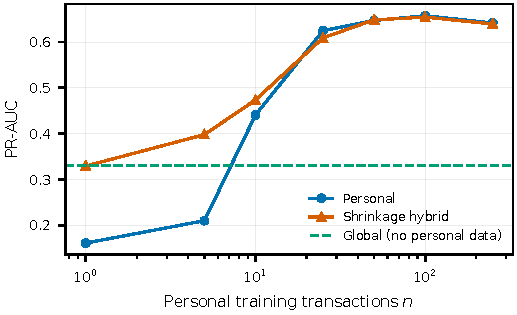
\includegraphics[width=\columnwidth]{figures/fig_arms.pdf}
\caption{Personal, population (global) and shrinkage-hybrid Mahalanobis detectors on Berka. The personal model falls below the global model until $n\approx10$; the hybrid starts at the global level, tracks or exceeds the personal model at every $n$ below 25, and is indistinguishable from it from $n=25$ on.}
\label{fig:arms}
\end{figure}

\begin{table}[!t]
\caption{Mahalanobis on Berka: personal versus global (constant PR-AUC 0.330) and shrinkage hybrid versus personal, paired over 300 accounts. All personal-versus-global Holm $p<0.001$. Final column: hybrid minus personal (Holm $p$).}
\label{tab:arms}
\centering\footnotesize\setlength{\tabcolsep}{2.6pt}
\begin{tabular}{r cc cc}
\toprule
$n$ & Personal & Hybrid & Pers.\ $-$ Global [95\% CI] & Hyb.\ $-$ Pers.\ ($p$) \\
\midrule
1   & 0.161 & 0.329 & $-0.169$ [$-0.196$, $-0.142$] & $+0.168$ ($<$0.001) \\
5   & 0.210 & 0.398 & $-0.120$ [$-0.144$, $-0.096$] & $+0.188$ ($<$0.001) \\
10  & 0.441 & 0.474 & $+0.111$ [$+0.082$, $+0.140$] & $+0.033$ (0.078) \\
25  & 0.625 & 0.609 & $+0.295$ [$+0.265$, $+0.324$] & $-0.016$ (0.795) \\
50  & 0.647 & 0.648 & $+0.317$ [$+0.290$, $+0.345$] & $+0.001$ (1.000) \\
100 & 0.657 & 0.654 & $+0.327$ [$+0.299$, $+0.355$] & $-0.003$ (1.000) \\
250 & 0.642 & 0.639 & $+0.311$ [$+0.284$, $+0.338$] & $-0.002$ (1.000) \\
\bottomrule
\end{tabular}
\end{table}

A population model built from other people's data beats the person's own history below a crossover that depends on the detector. For Mahalanobis the personal model is worse than the global model through $n=5$ (rank-biserial effect $-0.544$) and better from $n=10$ ($+0.465$, \cref{tab:arms}). For $k$-NN, with a global PR-AUC of 0.465, the personal model is worse through $n=25$ ($-0.261$, effect $-0.883$) and better from $n=50$ ($+0.059$, rising to $+0.145$ at 250). At each of the five cohort seeds personal Mahalanobis first exceeds the global model at exactly $n=10$, even though the global model's own mean PR-AUC varies with the donor draw from 0.262 to 0.330. Personalisation is therefore not a safe default in the sparse regime.

The shrinkage hybrid removes the cold-start penalty (\cref{fig:arms,tab:arms}). It improves on the personal model by 0.168 at $n=1$ and 0.188 at $n=5$, and from $n=25$ no difference is detectable (Holm $p\ge0.795$, differences at most 0.016). It is never detectably worse than the personal model and never meaningfully below the global model. The weight $n/(n+\kappa)$ removes the penalty at no measurable cost at large $n$.

\paragraph{Where hybridisation fails}
In the simulation the hybrid plateaus at PR-AUC 0.401 while the personal model reaches 0.924. The simulation's strongest features are personal novelty indicators (is this merchant one \emph{you} have used), computed against a reference history; the hybrid computes them against the population reference, which destroys the signal that matters. Parameter shrinkage cannot recover information the feature representation has already discarded. Shrinkage hybrids therefore reduce the personal data requirement when the personal signal lives in the \emph{parameters} of a shared representation, as in the Berka features, and fail when it lives in the representation itself, as in the simulation's.

\subsection{The Operating Point Depends on the Calibration Rule}\label{sec:calibration}

PR-AUC measures ranking; a deployed detector also needs an alert threshold. \Cref{tab:calib} compares the two calibration rules of \cref{sec:protocol} for personal Mahalanobis on the primary cohort.

\begin{table}[!t]
\caption{Personal Mahalanobis on Berka under in-sample and leave-one-out (LOO) calibration (nominal FPR 0.05; 300 accounts). At $n=1$ the in-sample rule flags 99.9\% of transactions and the LOO rule is undefined.}
\label{tab:calib}
\centering\footnotesize\setlength{\tabcolsep}{2.8pt}
\begin{tabular}{r cc cccc}
\toprule
& \multicolumn{2}{c}{In-sample} & \multicolumn{4}{c}{LOO} \\
\cmidrule(lr){2-3}\cmidrule(lr){4-7}
$n$ & Flag rate & FPR & Flag rate & FPR & Recall & Precision \\
\midrule
5   & 0.989 & 0.988 & 0.152 & 0.151 & 0.163 & 0.110 \\
10  & 0.960 & 0.956 & 0.012 & 0.007 & 0.058 & 0.667 \\
25  & 0.391 & 0.335 & 0.110 & 0.066 & 0.503 & 0.577 \\
50  & 0.251 & 0.189 & 0.126 & 0.073 & 0.612 & 0.558 \\
100 & 0.196 & 0.134 & 0.134 & 0.076 & 0.658 & 0.533 \\
250 & 0.162 & 0.104 & 0.136 & 0.080 & 0.647 & 0.516 \\
\bottomrule
\end{tabular}
\end{table}

\paragraph{In-sample calibration flags almost everything at small $n$}
At $n=10$ the PR-AUC is 0.441, more than four times the prevalence baseline, yet the in-sample rule flags 96\% of all transactions. The cause is a bias in the rule, not data scarcity. In-sample scores are biased low by construction whenever a model scores the points it was fitted to: a personal Mahalanobis fit on $n\le d=21$ points has a singular covariance, so every training point lies in the span of the fit and scores near zero, and a $k$-NN training point counts itself as a neighbour at distance 0. The 95th percentile of such scores is systematically too low, and more data removes that bias only slowly.

\paragraph{LOO calibration makes the detector silent at $n=10$ and near-nominal from $n=25$}
Under LOO calibration, which is out-of-sample, the same detector flags 1.2\% of transactions at $n=10$ with recall 0.058: ten LOO scores give a threshold dominated by the single most extreme of them. From $n=25$ the FPR is 0.066 against a nominal 0.05, rising slowly to 0.080 at $n=250$, with recall between 0.50 and 0.65. The paired in-sample-minus-LOO difference in FPR is significant at every size (Wilcoxon $p<10^{-36}$), with mean differences of 0.949 at $n=10$, 0.268 at 25 and 0.116 at 50. The PR-AUC at $n=10$ still does not translate into a usable operating point: the detector is silent, not noisy, for as long as its threshold must come from the person's own ten points. The nominal 5\% is missed by 1.6 to 3 points at every size from 25; training points and evaluation-window points are not exchangeable, since the window is later in time, and we did not diagnose the cause, so ``near-nominal'' is not ``well calibrated''.

\begin{table*}[!t]
\caption{Mean FPR under LOO calibration, with the in-sample value in parentheses (nominal 0.05). Six personal detectors and the shrinkage-hybrid Mahalanobis on Berka, 300 accounts at each of five cohort seeds (1{,}500 account-seed rows per cell). Recall under LOO calibration is in \cref{tab:recall}.}
\label{tab:fpr_all}
\centering\footnotesize\setlength{\tabcolsep}{5pt}
\begin{tabular}{l cccccc}
\toprule
Detector & $n=5$ & $n=10$ & $n=25$ & $n=50$ & $n=100$ & $n=250$ \\
\midrule
Gaussian z       & 0.049 (0.263) & 0.012 (0.108) & 0.005 (0.017) & 0.006 (0.007) & 0.007 (0.007) & 0.006 (0.007) \\
Robust z         & 0.045 (0.237) & 0.048 (0.104) & 0.017 (0.016) & 0.013 (0.006) & 0.012 (0.006) & 0.009 (0.006) \\
Mahalanobis      & 0.154 (0.989) & 0.012 (0.958) & 0.066 (0.331) & 0.068 (0.185) & 0.073 (0.132) & 0.083 (0.107) \\
$k$-NN           & 0.492 (0.492) & 0.132 (0.194) & 0.041 (0.098) & 0.054 (0.104) & 0.071 (0.105) & 0.082 (0.111) \\
Isolation Forest & 0.535 (0.236) & 0.205 (0.199) & 0.009 (0.143) & 0.025 (0.113) & 0.042 (0.090) & 0.055 (0.075) \\
Autoencoder      & 0.191 (0.984) & 0.021 (0.667) & 0.049 (0.205) & 0.060 (0.127) & 0.068 (0.100) & 0.077 (0.091) \\
Hybrid           & 0.097 (0.395) & 0.028 (0.266) & 0.040 (0.184) & 0.060 (0.138) & 0.070 (0.114) & 0.080 (0.102) \\
\bottomrule
\end{tabular}
\end{table*}

\paragraph{The effect holds across detectors and cohorts, and its direction varies}
Repeating the comparison for all six personal detectors and the hybrid at the five seeds (\cref{tab:fpr_all}) shows the following.
\begin{itemize}
\item \emph{The Mahalanobis correction is stable across cohorts.} Pooled over five seeds, FPR is 0.012 at $n=10$ and 0.066 at $n=25$, and the across-seed standard deviation of the per-seed mean FPR is at most 0.008 at any size from 5.
\item \emph{The artefact is not specific to Mahalanobis.} The autoencoder's in-sample flag rate at $n=10$ is 0.691 against 0.025 under LOO; the hybrid's is 0.296 against 0.051. In-sample and LOO FPR differ significantly (paired Wilcoxon $p<10^{-4}$) in 39 of 42 detector-by-size cells; the in-sample FPR is higher in 35 and lower in 4 (Isolation Forest at $n=5$; robust $z$ at $n=50$, 100 and 250). The three cells without a detectable difference are Isolation Forest at $n=10$, robust $z$ at $n=25$, and $k$-NN at $n=5$, where the two rules are identical by construction: with $k=n=5$ the in-sample fifth-nearest-neighbour distance, counting the point itself at distance 0, equals the maximum distance to the other four points, which is the LOO score.
\item \emph{A usable operating point near $n=25$ holds only for detectors that also rank well.} At $n=25$ the FPRs of Mahalanobis (0.066), the autoencoder (0.049) and the hybrid (0.040) lie within about 1.6 points of 0.05, with recall 0.37 to 0.50. The $k$-NN detector has FPR 0.041 but recall 0.038 at $n=25$ and stays silent until about $n=50$ (recall 0.386). Isolation Forest has FPR 0.009 and recall 0.018 at $n=25$ and reaches recall of only 0.236 at $n=250$, so no usable operating point appears within the sizes tested, consistent with its PR-AUC curve. The two $z$-score detectors are conservative under LOO and keep recall between 0.035 and 0.055 at every $n\ge25$.
\item \emph{The in-sample rule is not an upper bound on false-positive burden.} Isolation Forest flags more under LOO than in-sample at $n=5$ (flag rate 0.533 against 0.232), the two rules are indistinguishable at $n=10$ (paired $p=0.7$), and robust $z$ has a slightly lower in-sample FPR at $n\ge50$ (by 0.003 to 0.007). The LOO forest is fitted on $n-1$ points and an isolation forest's score normalisation depends on its subsample size, so its LOO scores and the scores of the $n$-point forest are not on exactly the same scale; whether this explains Isolation Forest at $n\le10$ is untested, and that behaviour is not evidence about the detector.
\item \emph{The hybrid has the best small-$n$ operating behaviour.} At $n=10$ its LOO FPR is 0.028 and recall 0.254, against 0.012 and 0.055 for personal Mahalanobis; at $n=5$ the figures are 0.097 and 0.272 against 0.154 and 0.168. This extends the ranking result of \cref{sec:arms} to the operating point; it is an observation from one calibration rule and one anomaly protocol, not a pre-specified significance test.
\end{itemize}

\paragraph{Consequence for the sufficiency threshold}
The measured requirement depends on how the threshold is calibrated as well as on the criterion. Under in-sample calibration the Mahalanobis FPR is still 0.189 at $n=50$ and 0.104 at $n=250$; under LOO calibration it lies within about 3 points of nominal from $n=25$ for Mahalanobis, the autoencoder and the hybrid, but only from about $n=50$ for $k$-NN and not within 250 for Isolation Forest. Any single-number ``$N$ transactions is enough'' claim conceals both the criterion and the calibration rule. The relative-90 ranking thresholds of \cref{tab:thresholds} depend on no threshold rule. Operating-point results for the global arm, Protocol~P, the temporal experiments, the simulation, TabFormer and the audit of \cref{sec:audit} at $n=10$ and 50 use the in-sample rule; because that rule is not an upper bound, they are not worst-case figures either.

\subsection{Recency, Volume and Drift}\label{sec:recency}

Does more history help because of the count of transactions or the span of time they cover? We hold the count at $n=50$ and widen coverage by stride-sampling the history. Inter-arrival gaps are computed against each transaction's true position in the unthinned timeline, so thinning does not change the gap feature's meaning.

\begin{table}[!t]
\caption{Fixed count $n=50$, widening temporal coverage (Berka, 300 accounts). Stride~1 is the 50 most recent transactions; $\Delta$ is the paired PR-AUC difference from stride~1.}
\label{tab:stride}
\centering\footnotesize\setlength{\tabcolsep}{4pt}
\begin{tabular}{l c cc cc}
\toprule
 & Median & \multicolumn{2}{c}{Mahalanobis} & \multicolumn{2}{c}{$k$-NN} \\
\cmidrule(lr){3-4}\cmidrule(lr){5-6}
Arm & span (days) & PR-AUC & $\Delta$ & PR-AUC & $\Delta$ \\
\midrule
Stride 1 & 224 & 0.663 & --- & 0.540 & --- \\
Stride 2 & 457 & 0.660 & $-0.004$ & 0.478 & $-0.062$ \\
Stride 4 & 946 & 0.627 & $-0.036$ & 0.430 & $-0.110$ \\
\bottomrule
\end{tabular}
\end{table}

\Cref{tab:stride} shows that for Mahalanobis stride 2 changes PR-AUC by $-0.004$ (not detectable, $p=0.304$) and stride 4 by $-0.036$ ($p<0.001$, effect $-0.300$); for $k$-NN both strides lose significantly ($p<0.001$). Coverage and sampling density cannot be varied independently at fixed count: a control arm that keeps the 50 transactions recent but thins them by four necessarily reaches back four times further, and it did (span 950 against 946 days, near-identical results). The effect of span is therefore not separable from the effect of density in this design. Together with \cref{sec:curves} the evidence is clear on one point: raising the count from 50 to 250 at natural density changes Mahalanobis PR-AUC from 0.647 to 0.642, while drawing the same 50 transactions from a span four times longer costs 0.036. Within Berka, neither more transactions nor more time helps once about 50 recent transactions are available, and reaching further back is mildly harmful: recency dominates volume.

\paragraph{Drift does not explain the cost of older history}
Behavioural drift is the natural explanation, so we test it directly. For each account, drift is the Mahalanobis distance between the 150 transactions added when history grows from 100 to 250 and the 100 transactions already present at $n=100$, measured in the account's own recent coordinate system: both blocks are mapped to the detectors' causal features, standardised by a scaler fitted on the recent block only, and compared through the recent block's ridge-regularised covariance. This is ``how many of my own recent standard deviations away is my older behaviour'', computed independently of any detector score or anomaly label. Drift is substantial and accumulates with lag: its median is 0.69 and mean 1.00 (maximum 12.6), and a lag sweep shows mean drift rising from 0 at lag 0 to 1.72 at lag 25 and plateauing near 3.2 to 3.6 by 150 to 200 transactions back. Older behaviour does look different from recent behaviour. But an account's drift magnitude does not predict that account's own marginal PR-AUC gain from 100 to 250 transactions: Spearman $\rho=-0.081$ for Mahalanobis and $+0.070$ for $k$-NN (both Holm $p=0.32$, $n=300$). Drift accumulates with lag, yet it does not explain which accounts lose performance when older history is added. The mechanism behind the negative $100\to250$ step, and behind the cost of reaching further back, remains open.

\subsection{Robustness to the Anomaly Definition}\label{sec:robust}

Under Protocol~P (amount multiplied by 5), the ordering of detectors changes. The Gaussian-$z$ detector, flat under Protocol~I (0.166 at $n=100$), becomes competitive (0.294), as expected for a perturbation applied to amount alone. Mahalanobis remains best but at a lower level (0.455 at $n=100$, against 0.657), with PR-AUC 0.258, 0.423 and 0.453 at $n=1$, 25 and 250; $k$-NN reaches 0.153, 0.212 and 0.217 and Isolation Forest 0.163, 0.194 and 0.211 at $n=25$, 100 and 250. The Mahalanobis relative-90 threshold is again 25. The threshold of roughly 25 transactions therefore holds across two structurally different anomaly definitions, while the \emph{level} of achievable PR-AUC is strongly protocol-dependent and does not transfer between them.

\subsection{Behavioural Variability and the Requirement}\label{sec:variability}

\begin{figure}[!t]
\centering
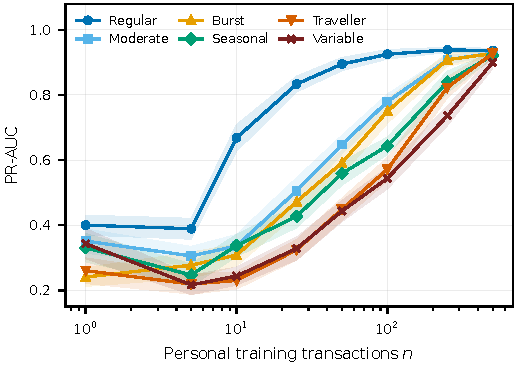
\includegraphics[width=\columnwidth]{figures/fig_sim_archetypes.pdf}
\caption{Simulation: personal Mahalanobis PR-AUC by behavioural archetype (mean $\pm$ 1.96 standard errors over 40 individuals per archetype). The regular archetype saturates by $n\approx50$; traveller and variable individuals need several hundred transactions, yet all archetypes converge to similar ceilings.}
\label{fig:sim}
\end{figure}

\begin{table}[!t]
\caption{Simulation: relative-90 threshold and best PR-AUC of personal Mahalanobis by archetype.}
\label{tab:archetypes}
\centering\footnotesize\setlength{\tabcolsep}{6pt}
\begin{tabular}{l cc}
\toprule
Archetype & Rel-90 threshold & Best PR-AUC \\
\midrule
Regular   & 50  & 0.939 \\
Moderate  & 250 & 0.929 \\
Seasonal  & 250 & 0.923 \\
Burst     & 250 & 0.927 \\
Traveller & 500 & 0.928 \\
Variable  & 500 & 0.900 \\
\bottomrule
\end{tabular}
\end{table}

\paragraph{Under controlled manipulation, variability predicts the requirement}
With variability set by the generative parameters, every descriptor predicts each individual's relative-90 threshold (all Holm $p<0.001$): number of distinct merchants ($\rho=+0.708$), category entropy ($+0.700$), merchant entropy ($+0.700$), log-amount standard deviation ($+0.673$), location entropy ($+0.617$) and inter-arrival coefficient of variation ($+0.484$). The archetypes differ tenfold in requirement, from 50 to 500 transactions (\cref{fig:sim,tab:archetypes}), while converging to similar ceilings (best PR-AUC 0.900 to 0.939): variability changes the \emph{rate} of learning far more than its ceiling.

\paragraph{In real accounts, no descriptor predicts the requirement}
We computed eight descriptors on each Berka account's 250-transaction history (amount coefficient of variation, robust amount coefficient of variation, log-amount interquartile range, operation entropy, \texttt{k\_symbol} entropy, operation diversity, inter-arrival coefficient of variation and credit share) and correlated each with the account's own relative-90 threshold. After Holm correction over the eight, all $p\ge0.867$ and all $|\rho|\le0.12$. The test uses the 183 accounts with a defined threshold; the other 117 (39\%) never reached and held 90\% of their own best value, so the 183 are a non-random subset of better-behaved accounts. At that size a two-sided Spearman test reaches about 80\% power only for $|\rho|\gtrsim0.21$ before correction, so the null excludes moderate-to-strong effects and leaves weak ones open. Diverse operation and \texttt{k\_symbol} usage does correlate with higher \emph{best achievable} PR-AUC (uncorrected $\rho=+0.167$ to $+0.209$, $p=0.005$ to 0.024), plausibly because a distinctive profile is easier to separate from an impostor's.

\paragraph{Three explanations remain}
The Berka descriptors may be too thin: the dataset has no merchant, category or location channels, which are exactly the channels carrying the simulation's effect. The real cohort's variability range may be too narrow, since all accounts are ordinary retail accounts at one bank. Or observed variability may be confounded with account type, tenure and product mix in ways the simulation excludes by construction. The simulation shows that the effect exists when the generative parameters are what theory says they are; it is not evidence that the effect exists in real data. A partial test uses TabFormer, whose schema has the missing channels: there, state entropy does predict an entity's relative-90 threshold after Holm correction ($\rho=+0.19$, $p=0.028$; merchant diversity is marginal at $p=0.148$), unlike every descriptor on Berka. This is consistent with channel availability being what the Berka null lacked; because TabFormer is synthetic, it cannot turn the real-data null into a positive finding.

\paragraph{Anomaly classes differ in their data requirements}
In the simulation, the mean score percentile of Mahalanobis (1.0 is most anomalous) shows that categorical-novelty anomalies start near chance and improve steeply, since recognising an unfamiliar merchant requires having seen the familiar ones: merchant, category and geographic anomalies rise from 0.545, 0.547 and 0.642 at $n=1$ to 0.947, 0.957 and 0.969 at $n=250$. Amount and temporal anomalies start above chance (0.789 and 0.721) and improve least (0.861 and 0.845 at $n=250$), because one observation already locates a distribution's centre roughly. Multivariate anomalies are effectively saturated by $n=50$ (0.999). Amount detectability falls from 0.789 at $n=1$ to 0.576 at $n=10$ before recovering; the apparent competence at $n=1$ is an artefact of degenerate variance, not detection.

\subsection{Replication on a Second Dataset}\label{sec:tabformer}

\begin{figure}[!t]
\centering
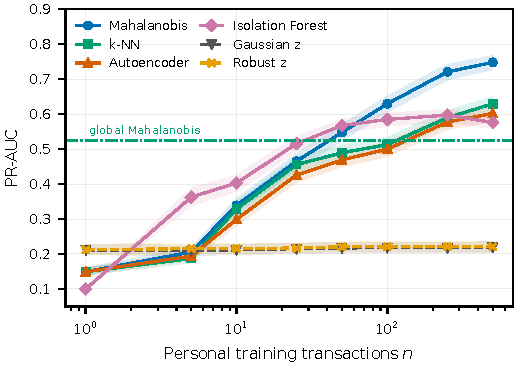
\includegraphics[width=\columnwidth]{figures/fig_tabformer_curves.pdf}
\caption{Data efficiency on TabFormer (\emph{synthetic} card data; Protocol~I; 300 entities; bands are 95\% bootstrap intervals). The steep-rise, early-plateau shape and the flat $z$-scores recur, but Isolation Forest is the best detector at $n=5$ to $50$, the opposite of its position on Berka.}
\label{fig:tabformer}
\end{figure}

Every number in this subsection comes from TabFormer, a synthetic dataset, and none is pooled with the real-data results. The question is whether the shape found on Berka (steep early rise, plateau, a global-personal crossover, an early and stable threshold) is specific to one dataset.

\paragraph{The shape replicates, with a later threshold}
Mahalanobis again rises steeply and attains the highest ceiling (0.748 at $n=500$), and both $z$-scores are flat at 0.21 to 0.22 at every size (\cref{fig:tabformer}). The Mahalanobis relative-90 threshold is 250, against Berka's 25. Two candidate reasons, both untested, are that TabFormer's 26-dimensional feature space needs more observations before an $n\le d$ covariance estimate stops being singular, and that the global model here is much stronger (PR-AUC 0.524 against Berka's 0.330), which raises the bar that the personal curve must clear to look saturated.

\paragraph{The global-personal crossover moves with the strength of the global model}
Personal Mahalanobis minus global is $-0.375$ at $n=1$, $-0.059$ at 25 (Holm $p<0.001$), $+0.023$ at 50 ($p=0.094$), $+0.105$ at 100 and $+0.223$ at 500 (both $p<0.001$). The crossover falls between $n=25$ and $100$, later than Berka's 5 to 10, as expected if a stronger population baseline raises the bar that personalisation must clear. Personalisation is harmful below a detector- and dataset-dependent crossover on both datasets.

\paragraph{Detector ranking under scarcity reverses}
On Berka, Isolation Forest is the worst detector at every history size, from PR-AUC 0.100 at $n=1$ (exactly the prevalence baseline) to 0.343 at 250, and its fitting is the most expensive: at $n=250$ the median fit time is 0.46\,ms for Mahalanobis, 5.0\,ms for $k$-NN, 22.9\,ms for the autoencoder and 156.3\,ms for Isolation Forest. On TabFormer it is the single best detector at $n=5$, 10, 25 and 50 (0.362 against Mahalanobis's 0.206 at $n=5$, and 0.567 against 0.548 at $n=50$) and falls behind Mahalanobis only from $n=100$ (0.585 against 0.630). A candidate explanation, untested, is that TabFormer's higher-dimensional, one-hot-heavy space gives isolation splits more structure to exploit at small samples. The answer to whether sophisticated detectors beat simple statistics under scarcity is therefore dataset-dependent: on Berka the best detector is a shrinkage-regularised covariance estimate, and on TabFormer the answer differs at small $n$.

\paragraph{Fraud labels could not be evaluated}
An exploratory protocol against the generator's own fraud label found no positive example: none of the 300 evaluated entities' 60-transaction windows contained a generator-labelled fraud, consistent with the 0.122\% corpus-wide prevalence (about 0.07 expected per window).

\subsection{Disparate-Impact Audit}\label{sec:audit}

Sparse-history users are the people the study is most about, so we test whether false-positive burden concentrates by district economics. We join the 300 evaluated accounts to their district's average salary, unemployment rate, urbanisation ratio and region, and test whether the personal Mahalanobis detector's FPR varies with them (Kruskal-Wallis across 8 regions; Spearman with Holm correction over the three continuous variables). The audit is ecological: Berka carries no per-person demographic field.

\begin{table}[!t]
\caption{Disparate-impact audit under LOO calibration (Berka, 300 accounts). Spearman $\rho$ between an account's FPR and its district's attribute (Holm $p$), and Kruskal-Wallis $p$ across regions. Mean FPR is 0.066, 0.073 and 0.076.}
\label{tab:audit}
\centering\footnotesize\setlength{\tabcolsep}{3pt}
\begin{tabular}{r ccc c}
\toprule
$n$ & Avg.\ salary & Unemployment & Urban ratio & Region \\
\midrule
25  & $-0.115$ (0.137) & $+0.012$ (0.838) & $-0.110$ (0.137) & 0.70 \\
50  & $-0.053$ (0.719) & $-0.026$ (0.719) & $-0.077$ (0.554) & 0.53 \\
100 & $-0.130$ (0.073) & $+0.104$ (0.145) & $-0.073$ (0.211) & 0.49 \\
\bottomrule
\end{tabular}
\end{table}

No relationship is Holm-significant (\cref{tab:audit}). Under the in-sample rule at $n=10$ and 50 all $|\rho|\le0.07$ and no Holm $p$ falls below 0.75; the $n=10$ half carries almost no information, because the in-sample FPR sits near its ceiling of 0.96 for every account. The salary correlation is negative at all three LOO sizes (higher-salary districts have somewhat lower FPR), with uncorrected $p=0.046$ at $n=25$ and 0.024 at $n=100$; with $|\rho|\le0.13$, at or below what 300 accounts can reliably detect (about 80\% power for $|\rho|\gtrsim0.16$), it is reported here as a trend, not an effect. False-positive burden is not visibly concentrated by district-level economic disadvantage in this dataset; whether it concentrates by age, tenure, immigration status or other axes that Berka cannot supply remains untested.
